\subsection{How to draw the robot}
\frame
{
  \frametitle{How to draw the robot}
  
  \emph{An exocentric vision system for \textit{3m.o.r.d.u.c.} 
    needs to tell \textit{R.E.A.R.} how to draw the robot itself,
    by subclassing \texttt{Robot} class.}
  \pause

  \vskip15pt

  \begin{block} {\alert{\texttt{Concrete classes}}}

    \pause
    \begin{itemize}
      
    \item \alert{\textit{Morduc}} \\
      3m.o.r.d.u.c. 3D model in \textit{OpenGL}
      \visible<3>{
        \begin{center}
          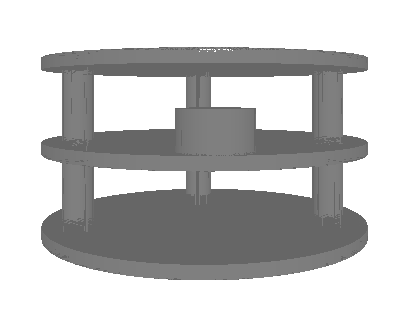
\includegraphics[width=80pt]{img/3morduc_opengl.png}
        \end{center}
      }
    \end{itemize}

  \end{block}
}

\subsection{How to choose the proper egocentric image}
\frame
{
  \frametitle{How to choose the proper egocentric image}
  
  \emph{An exocentric vision system for \textit{3m.o.r.d.u.c.} 
    needs to tell \textit{R.E.A.R.} how to choose the proper egocentric image,
    by implementig the \texttt{IImageSelector} interface.}
  \pause

  \vskip15pt

  \begin{block} {\alert{\texttt{Concrete classes}}}

    \begin{itemize}
      
    \pause
    \item \alert{\textit{SpacialMetricCalc}}
    \pause
    \item \alert{\textit{SweepMetricCalc}} \\
      details in next slide
    \pause
    \item \alert{\textit{AnotherSweepMetricCalc}} \\
      improvements of previous one, in order to
      provide user with more confortable teleguiding
      in case of strict turns

    \end{itemize}

  \end{block}
}

\subsubsection{Sweep Metric Algorithm}
\frame
{
  \frametitle{Sweep Metric Algorithm}
  
  \emph{Algorithm to choose the proper \textit{exocentric} image,
    among those collected.}
  \pause

  \begin{block} {\alert{\texttt{How it works}}}
    
    \begin{center}
      \visible<2->{
        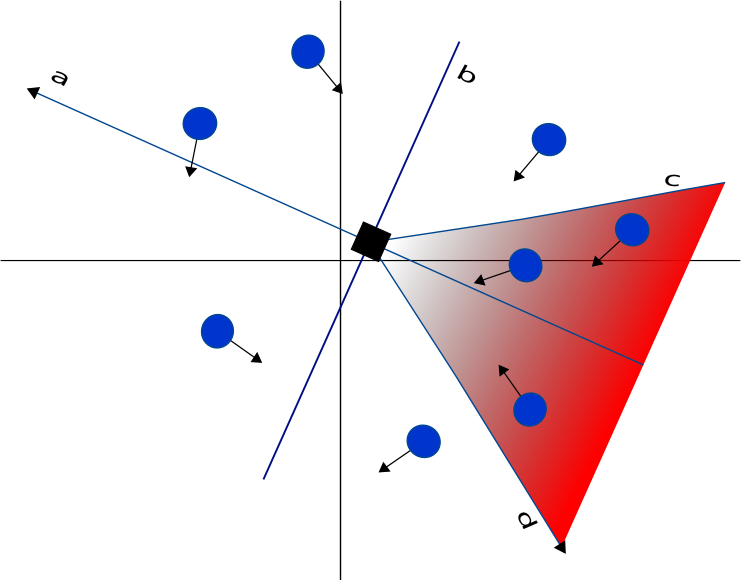
\includegraphics[width=150pt]{img/sma_1.png}
      }
    \end{center}
    
    \footnotesize{
      Explanation here.
    }
  \end{block}
}
